\documentclass{fkpset}

\usepackage{tikz-qtree,tikz-qtree-compat}
\usepackage{lscape}
\usepackage{caption}
\captionsetup[figure]{font=Large}
\lfoot{Due Monday, April 29\textsuperscript{th} 2019}
\begin{document}
\vspace{-1.9cm}
\begin{center}
  {\LARGE \scshape Math Forum Reflective Essay} \\[.5em]
  {\Large \scshape Forest Kobayashi}
\end{center}
\vspace{.8cm}

\begin{problem}[Prompt]
  Write a 750-1000 word reflective essay about your growth as a
  speaker in Math Forum. Successful essays will incorporate specific
  examples of lessons learned, together with accompanying allusions to
  your own talks as evidence. Readers of your essay should easily be
  able to sense the extent to which you have been engaged in Math
  Forum.\\

  Please note that the audience for your essay is primarily your
  instructor, but every member of the mathematics faculty should be
  able to read (and enjoy) your essay. Finally, to submit your essay,
  please upload a PDF copy of your essay to your drop box, and please
  name your file lastname-essay.pdf.
\end{problem}
\begin{solution}[Response.]
  \setlength{\parindent}{2em}

  I've really enjoyed my time in Math Forum. I've learned a lot about
  public speaking, managing my verbal/physical tics, and presenting
  technical information in a non-interactive setting. Honestly, I wish
  there were a sequel course --- I'd be really excited to try my hand
  at a full-hour lecture format, or something like it. I guess I could
  always try to start making YouTube videos or something\ldots but
  yeah, anyways, here are some of my big takeaways from the class:
  \begin{enumerate}[label=\arabic*)]
    \item It is much harder for me to present a non-technical topic
      than it is for me to present something like a theorem.
    \item Giving a talk is a vastly different experience from
      presenting material in an interactive setting (e.g.\ tutoring).
      In the latter, you can sometimes rely on your audience to signal
      where you need to slow down, what isn't quite clear, and so on.
      Because talks are more static and non-interactive, you have to
      put in a \emph{lot} of work ahead-of-time to identify places
      where your audience could get lost. As such,
    \item Knowing how to explain a topic well is \emph{not} the same
      thing as knowing how to give a good presentation on it. The
      latter requires a lot more work, including (but not limited to)
      \begin{enumerate}
        \item doing extensive meta-analysis of your own understanding
          of the subject,
        \item compressing that understanding into an easily-digestible
          model that you want to communicate to your audience, and
        \item finding ways to efficiently translate that model to
          words, pictures, and any other medium of communication.
      \end{enumerate}
  \end{enumerate}
  I'll go in-depth on these points below, but first, here's a list of
  some smaller lessons I won't have time to talk about:
  \begin{multicols}{2}
  \begin{itemize}
    \item I didn't realize how quickly I talk sometimes
    \item I didn't realize how hard it can be to prepare something
      \emph{cohesive}
    \item I didn't realize how much harder it is to give non-technical
      exposition compared to techical exposition.
    \item I didn't know how short 10 minutes could be
    \item Talking in a presentation format is a lot harder than
      talking interpersonally. When other people aren't actively
      interjecting and/or giving you feedback in your presentation of
      material (i.e., asking questions, etc.), it's a lot harder to
      remember to pause and take a breath / break to let everybody
      think
    \item How important it is to scaffold information
    \item How it can be helpful to break down a complicated technical
      question into subquestions
    \item How it can often be more helpful to focus time on
      \emph{introducing} the problem as opposed to \emph{describing}
      it.
    \item Explanations should maybe be a bit recursive. And they
      should get technical maybe only at the leaves of the tree.
    \item Knowing how to explain a technical topic well $\neq$ knowing
      how to \emph{speak} well
  \end{itemize}
  \end{multicols}

  % One of the big lessons I've learned in Math Forum is that there's a
  % big difference between presenting material \emph{interactively} and
  % presenting it \emph{statically}.

  % One of the big lessons I've learned in Math Forum is just how
  % different giving a talk is when

  % Big points to touch on:

  \begin{figure}[h]
    \centering
    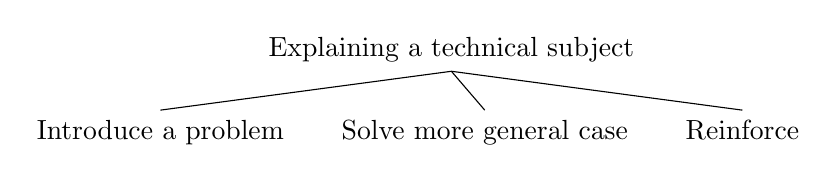
\begin{tikzpicture}[sibling distance=5mm]
      \Tree
      [.{Explaining a technical subject}
        [.{Introduce a problem} ]
        [.{Solve more general case} ]
        [.{Reinforce} ]
      ]
    \end{tikzpicture}
    \caption{Introducing a technical problem}
  \end{figure}
  \begin{landscape}
    \begin{figure}[p]
      \centering
      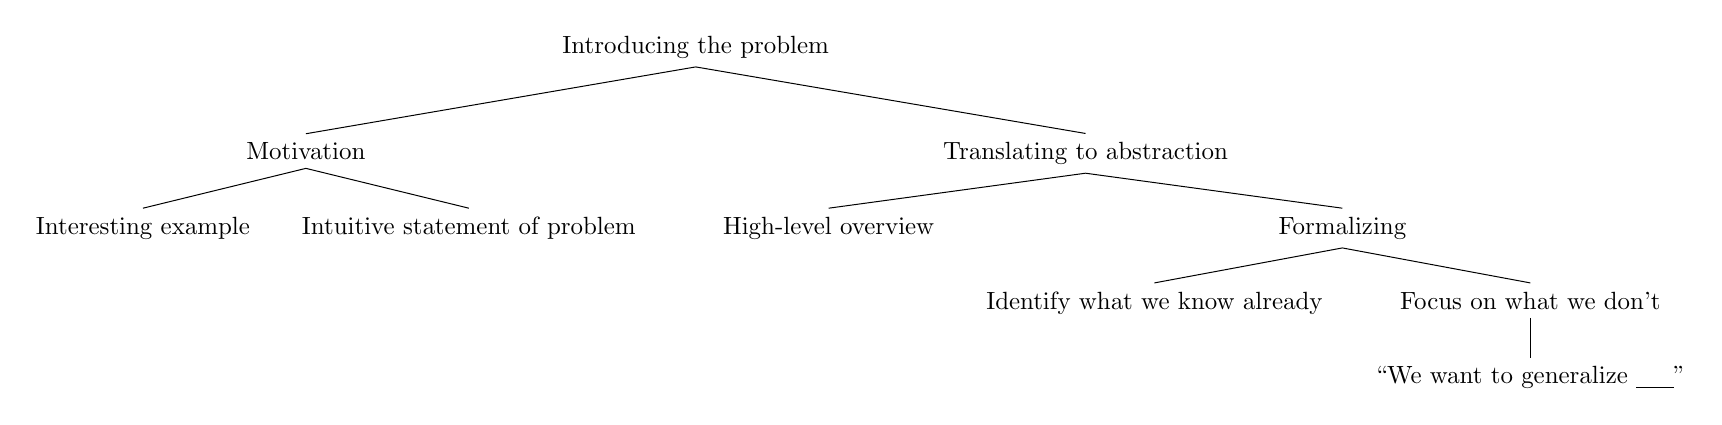
\begin{tikzpicture}[scale=.9, level 1/.style={level distance=1.5cm, sibling distance=10mm}, level 2/.style={sibling distance=5mm}, level 3/.style={sibling distance=5mm}]
        \Tree
        [.{Introducing the problem}
          [.{Motivation}
            [.{Interesting example} ]
            [.{Intuitive statement of problem} ]
          ]
          [.{Translating to abstraction}
            [.{High-level overview} ]
            [.{Formalizing}
              [.{Identify what we know already} ]
              [.{Focus on what we don't }
                [.{``We want to generalize \underline{\phantom{aaa}}''} ]
              ]
            ]
          ]
        ]
      \end{tikzpicture}
      \caption{Introducing a technical subject}
    \end{figure}
  \end{landscape}
  \begin{landscape}
    \begin{figure}[p]
      \centering
      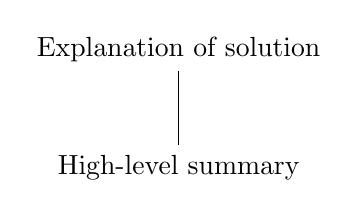
\begin{tikzpicture}[scale=1, level 1/.style={level distance=1.5cm, sibling distance=10mm}, level 2/.style={sibling distance=5mm}, level 3/.style={sibling distance=5mm}]
        \Tree
        [.{Explanation of solution}
          [.{High-level summary} ]
        ]
      \end{tikzpicture}
      \caption{Explaining the solution}
    \end{figure}
  \end{landscape}
\end{solution}



\end{document}
